%% Erläuterungen zu den Befehlen erfolgen unter
%% diesem Beispiel.

\documentclass{scrartcl}

\usepackage[utf8]{inputenc}
\usepackage[T1]{fontenc}
\usepackage{lmodern}
\usepackage[ngerman]{babel}
\usepackage{amsmath}
\usepackage{graphicx}
\usepackage{fancyhdr} %Header

\title{Verteiltes Genom Browsing}
\subtitle{Projektspezifikation}
%\author{Ben Schumacher, Malte Kruse}
\date{1. Dezember 2015}
\setkomafont{subtitle}{\bfseries \LARGE}
\renewcommand{\headrulewidth}{0pt}
%\date{6. September 2015}
\begin{document}
\pagestyle{fancy}
%\fancyhf{}
\cfoot{}
\rfoot{\pagemark}
\lhead{}
\rhead{}


\setcounter{page}{-1}
\maketitle
\thispagestyle{empty}
\newpage

\tableofcontents
\thispagestyle{empty}
\newpage

%\section{Einleitung}
%\newpage

\section{Integration}
\subsection{Integrationsprozess}
\subsubsection{Ablauf der Integration}
\subsubsection{Sequenzdiagramm}
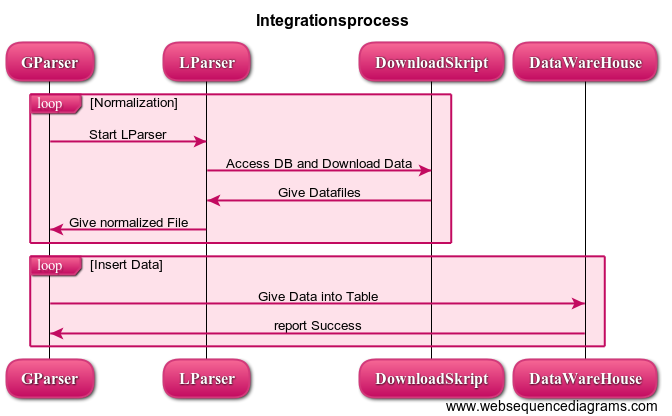
\includegraphics[width=\textwidth]{integration/SQDiag.png}
\subsection{Datenbankentwurf}
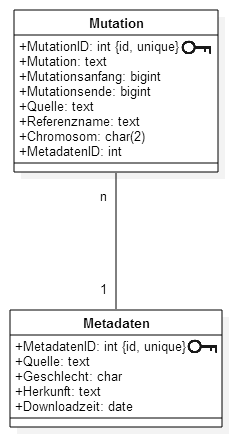
\includegraphics[width=\textwidth]{integration/DB.png}
%\subsubsection{Quellenauswahl}
%\subsubsection{Attributauswahl und -mapping}
%\subsubsection{Mengengerüst}
%\subsection{Parser}
%\subsubsection{Entwurf des Parsers}
%\subsubsection{UML-Diagramm}
%\subsection{Schnittstellenspezifikation}
%\subsubsection{Schnittstelle: Integration - Middleware}
%\subsubsection{Schnittstelle: Integration - Benutzer}
%\subsection{Komponententests}
%\subsubsection{Unit-Tests}
\newpage

\section{Middleware}
%\subsection{Indexstruktur}
%\subsubsection{Formale Beschreibung}
%\subsubsection{Komplexitätsabschätzung}
\subsection{UML-Diagramm}
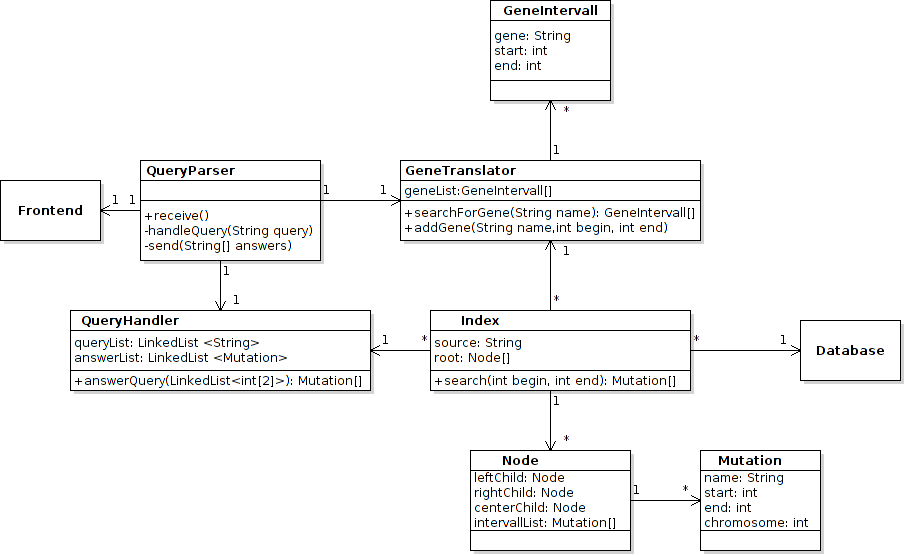
\includegraphics[width=\textwidth]{middleware/Middleware_Model_2nd_Revision.png}
%\subsubsection{Operationen als Pseudocode}
\subsection{Schnittstellenspezifikation: Middleware - Frontend}
\subsection{Unit-Tests}
\subsubsection{QueryHandler}
\subsubsection{GeneTranslator}
\newpage
\subsubsection{Intervallbaum}
\textbf{1. Intervalle einfügen:}\\
Das Intervall muss im Baum an der richtigen Stelle eingefügt werden und der Baum muss gegebenenfalls neu balanciert werden (z.B. wie ein AVL-Baum).\\\\
Bsp.: Einfügen des Intervalls [12,15]\\\\
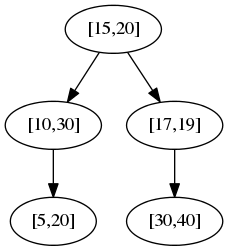
\includegraphics[width=0.2\textwidth]{middleware/Testfaelle/1.png}$~~~~~~~~~~~$
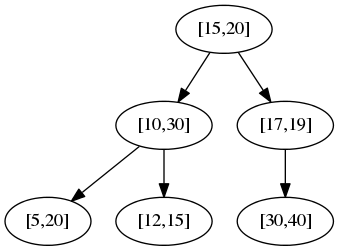
\includegraphics[width=0.3\textwidth]{middleware/Testfaelle/2.png}\\\\
\textbf{2. Intervall mit Startpunkt $>$ Endpunkt einfügen:}\\
Wenn ein Intervall (S,E) mit S$>$E eingefügt wird, dann sollte unser Programm eine Fehlermeldung ausgeben und darauf hinweisen, dass die Grenzen für das Intervall nicht korrekt sind.\\\\
Bsp.: Einfügen des Intervalls [20,10] in einen beliebigen Baum.\\\\
\textbf{3. Intervall mit Start- bzw. Endpunkt außerhalb des betrachteten Zahlenbereichs:}\\
Wenn ein Intervall in dem Baum eingefügt werden soll, das teilweise oder vollständig außerhalb unseres Zahlenbereichs liegt (Länge des Genoms), dann muss es eine Fehlermeldung geben, die dem Nutzer mitteilt, dass der gültige Zahlenbereich überschritten wurde.\\\\
Bsp.: Einfügen des Intervalls [-5,7] in einen beliebigen Baum.\newpage\hfill\\
\textbf{4. Schon vorhandenes Intervall einfügen:}\\
Duplikate sollen von unserem Baum nicht gespeichert werden, d.h. es wird kein neuer Knoten hinzugefügt, sondern die Informationen (bei uns also Pointer auf Dateien) des neuen Knotens müssen im bereits vorhandenen Knoten mitgespeichert werden.\\\\
Bsp.: Einfügen des Intervalls [15,20] in den folgenden Baum\\\\
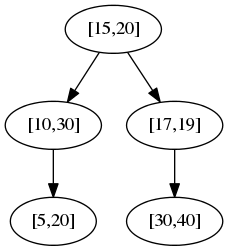
\includegraphics[width=0.2\textwidth]{middleware/Testfaelle/1.png}\\
\textbf{5. Intervalle löschen:}\\
Das Intervall soll aus dem Baum gelöscht werden und der Baum muss falls nötig wieder neu balanciert werden.\\\\
Bsp.: Löschen des Intervalls [10,30]\\\\
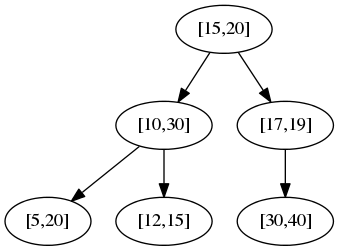
\includegraphics[width=0.3\textwidth]{middleware/Testfaelle/2.png}$~~~~~~~~~~~$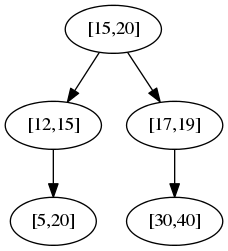
\includegraphics[width=0.2\textwidth]{middleware/Testfaelle/4.png}\\\\
\textbf{6. Nicht vorhandenes Intervall löschen:}\\
Versucht der Nutzer ein nicht im Baum gespeichertes Intervall zu löschen, so muss der Baum unverändert bleiben. Es kann zusätzlich darauf hingewiesen werden, dass der Knoten nicht existiert.\\\\
Bsp.: Löschen des Intervalls [50,60] aus dem folgenden Baum\\\\
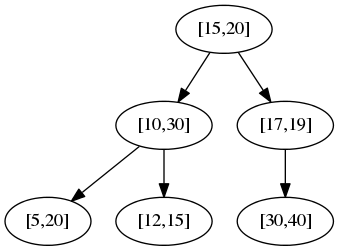
\includegraphics[width=0.3\textwidth]{middleware/Testfaelle/2.png}\\\\
\textbf{7. Suche nach vorhandenem Intervall:}\\
Bei der Suche sollen alle Intervalle ausgegeben werden, die das gesuchte Intervall in irgendeinem Punkt überlappen.\\\\
Bsp.: Suche im folgenden Baum\\\\
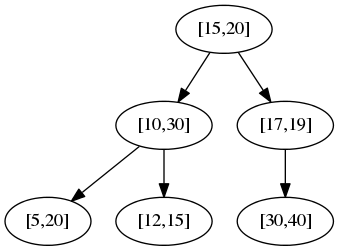
\includegraphics[width=0.3\textwidth]{middleware/Testfaelle/2.png}\\\\Suche [4,5] $\Rightarrow$ gib [5,20] aus\\
Suche [25,35] $\Rightarrow$ gib [10,30] und [30,40] aus\\
Suche [20,20] $\Rightarrow$ gib [15,20] und [5,20] aus
\subsection{Stresstests}
Beim Stresstest geht es darum das System so stark auszulasten wie mglich, um
zu sehen, ob die Antwortzeit für einzelne Clients, die Anfragen senden bei oer
Last merklich länger wird.\\
Hierfür werden Anfragen konstruiert, die so viel Arbeitslast wie mglich erzeugen.
In diesem Fall soll jeder Client Anfragen stellen, die in allen Quellen suchen;
Dadurch lastet jeder Client mit einer Anfrage alle VM’s aus. Weiterhin soll jeder
Client eine Gensuche anfragen, damit alle Anfragen den Extra-Schritt ber den
GeneTranslator machen mssen, was dazu führt, dass alle System-Komponenten
getestet werden. Auerdem kann so ein mglicher Flaschenhals in Form der
searcForGene()-Funktion entdeckt werden.\\
Da die Software eine sehr spezialisierte Suchmaschine ist, wird der Kreis an
Nutzern, die gleichzeitig den Webdienst in Anspruch nehmen relativ berschaubar
bleiben.\\
Die Idee ist deshalb in Erfahrung zu bringen, was der Kunde fr eine Nutzer-
menge für realistisch ählt. Wir setzen ersteinmal eine Zahl von 20 Clients fest.
Diese kann so weit erhht werden, bis eine merkliche Verlangsamung des Systems
eintritt.\\
Zusammenfassung:\\
20 Clients\\
Gennamen-Anfragen\\
Anfragen für alle Quellen\\
\newpage

\section{Frontend}
\subsection{Mock-Ups der Benutzerschnittstelle}
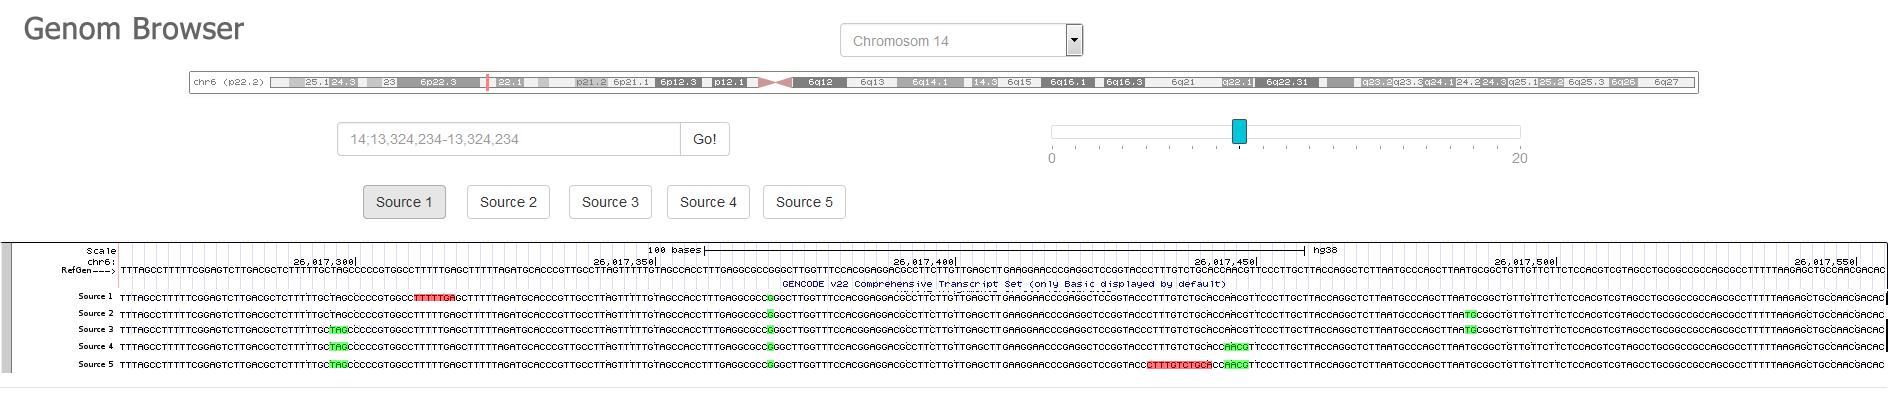
\includegraphics[width=\textwidth]{gui/gb_mockup_detail_view.png}
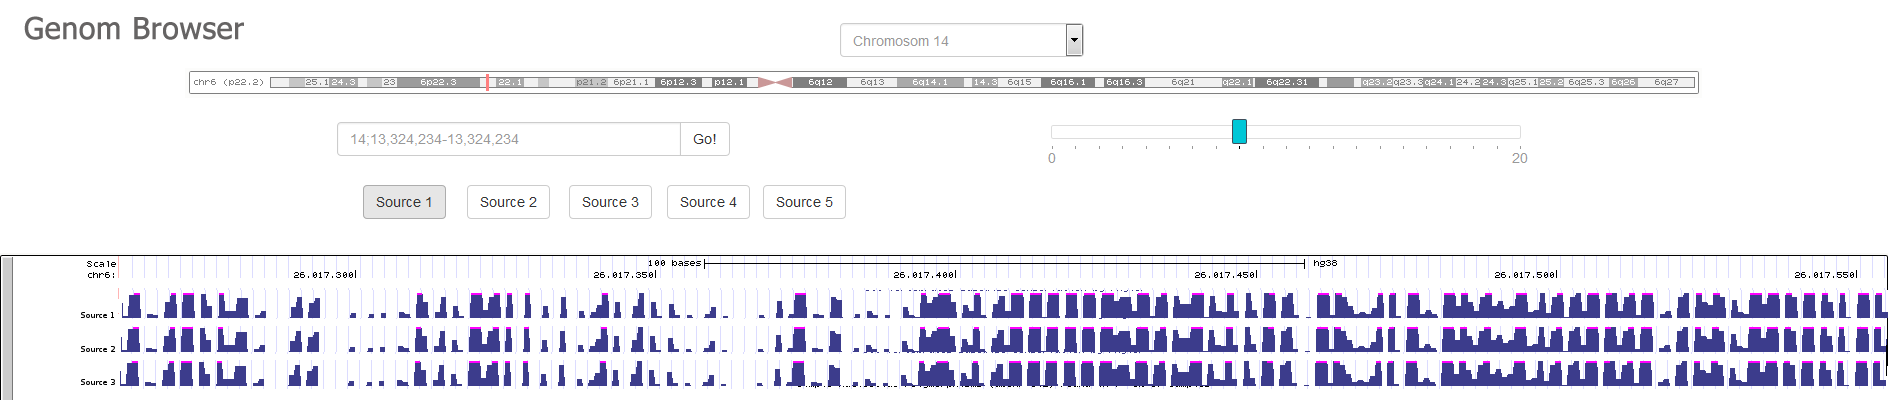
\includegraphics[width=\textwidth]{gui/gb_mockup_index_view.png}
\subsection{Klassen-Diagramm}
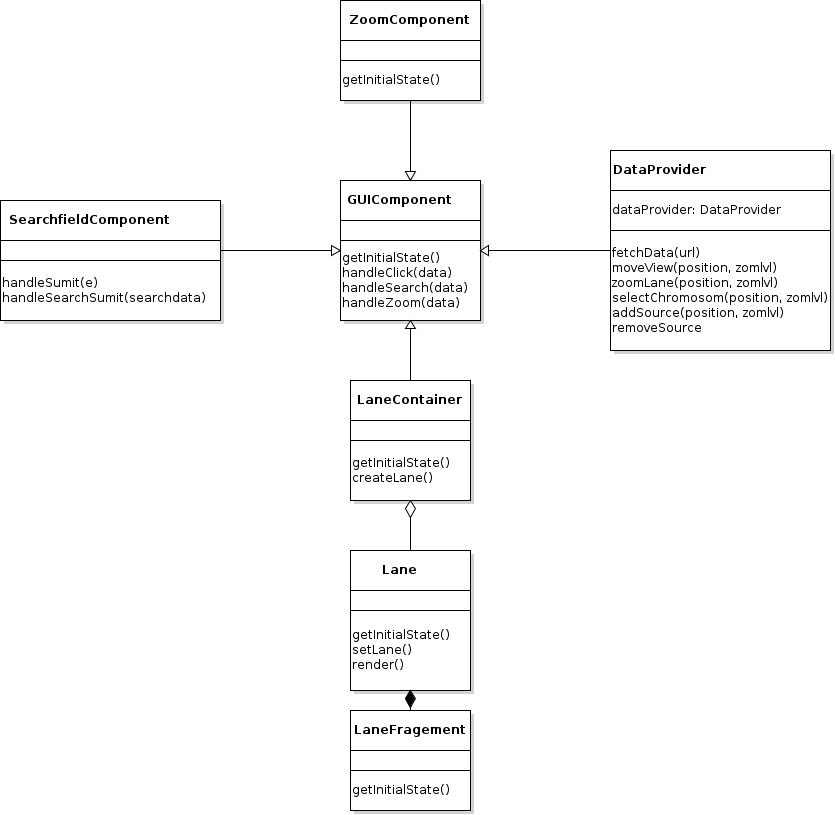
\includegraphics[width=\textwidth]{gui/gui-klassendiagramm.png}
\subsection{Sequenzdiagramm}
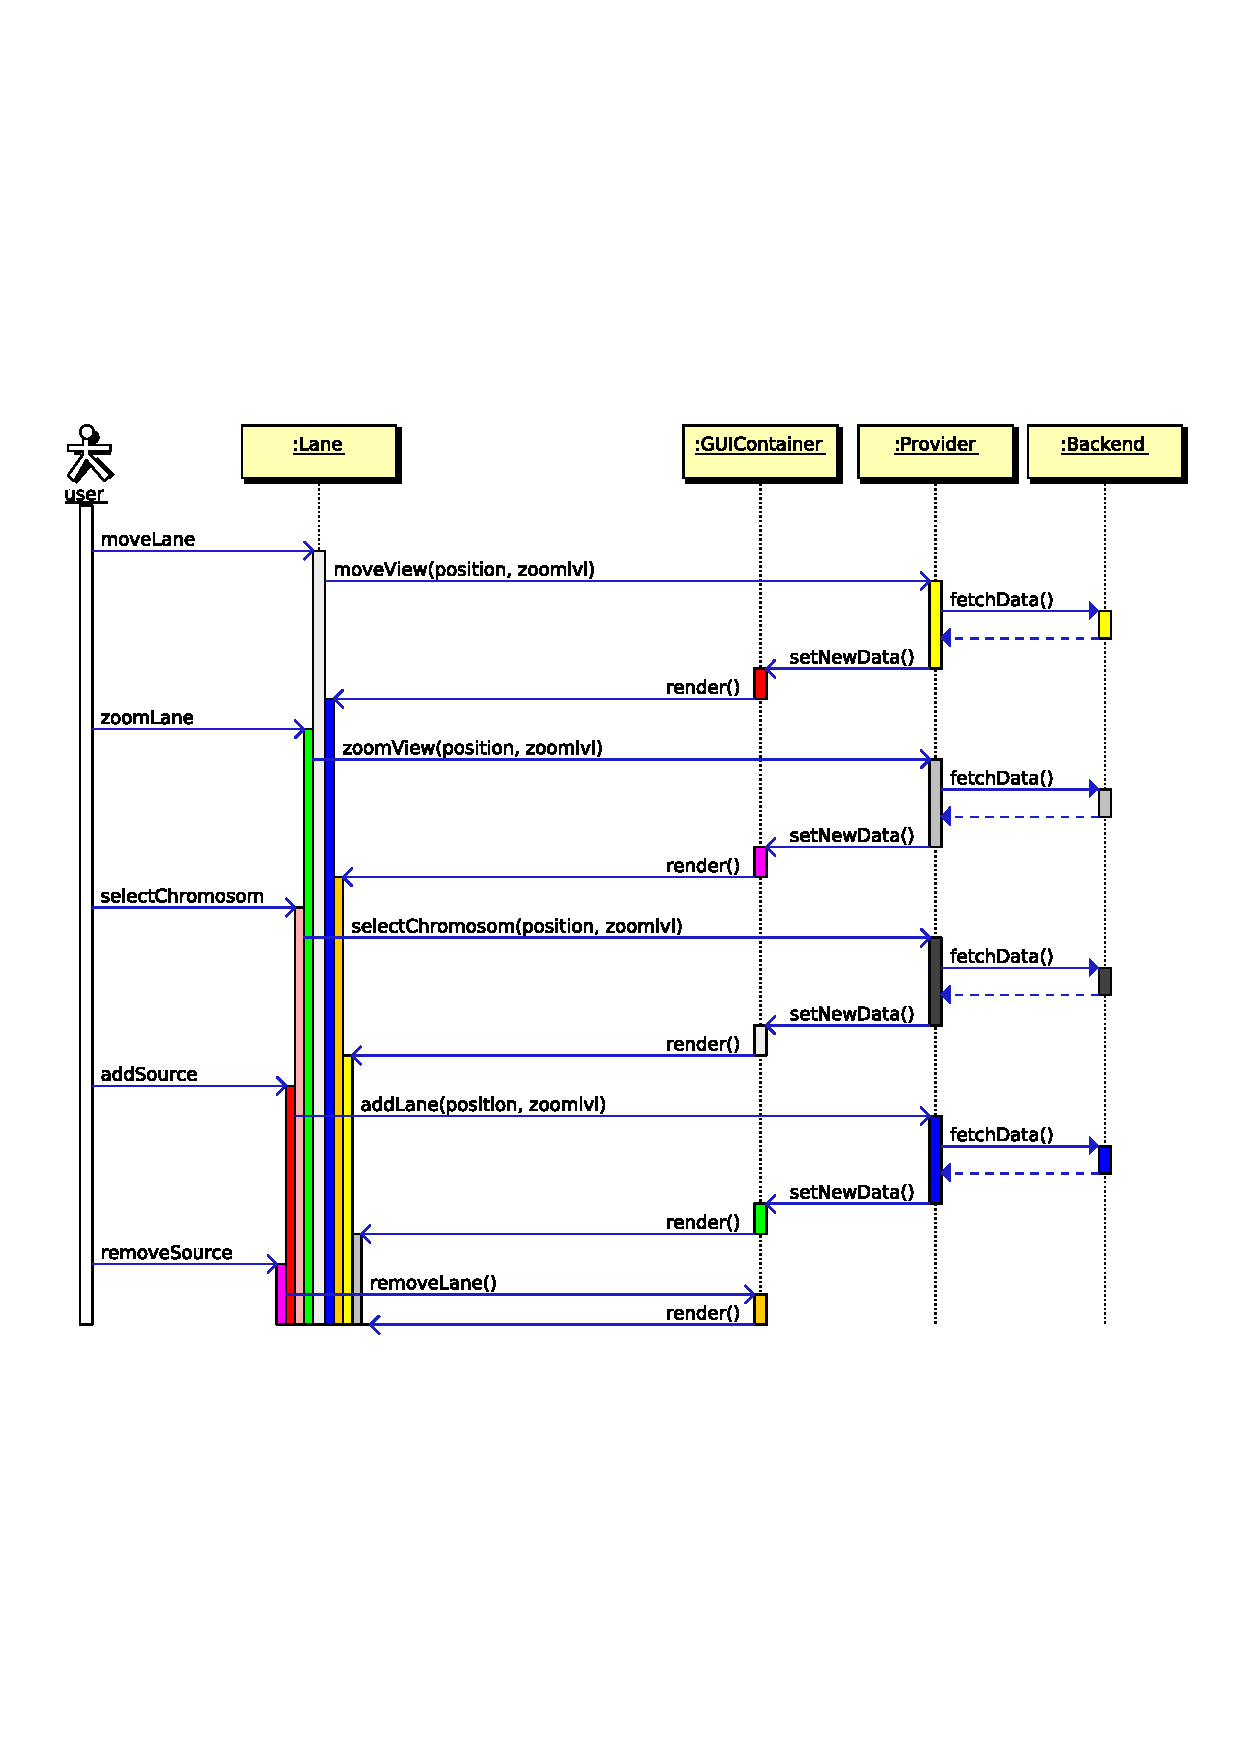
\includegraphics[width=\textwidth]{gui/GUI_Sequenzdiagramm.pdf}
\subsection{Use Cases}
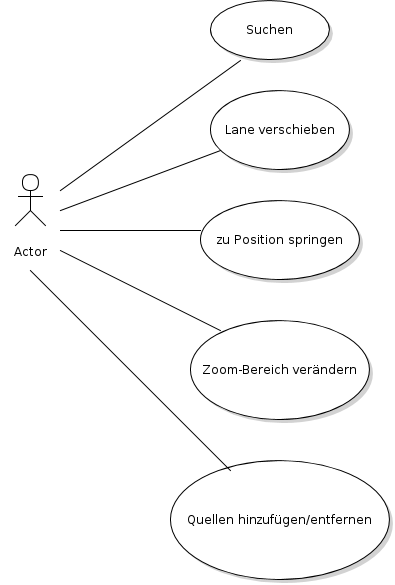
\includegraphics[width=\textwidth]{gui/gui-usecasediagramm.png}
%\subsection{Komponententests}
%\subsubsection{Unit-Tests}
\newpage

%\section{Integrationstest}
%\subsection{Ablauf der Integrationstests}

\end{document}